\documentclass[aspectratio=169, 10pt]{beamer}

% ---------- Tema y colores ----------
\usetheme{default}
\usecolortheme{default}
\setbeamertemplate{navigation symbols}{}
\setbeamertemplate{footline}[frame number]
\setbeamertemplate{frametitle continuation}{}

\definecolor{StanfordRed}{RGB}{140,21,21}
\definecolor{LightGray}{RGB}{240,240,240}
\definecolor{AccentGreen}{RGB}{0,130,100}
\definecolor{UCMBlue}{RGB}{4, 171, 226}
\definecolor{UCMNavy}{RGB}{20, 65, 134}

\definecolor{mitblue}{RGB}{20, 65, 134}
\definecolor{mitgray}{RGB}{169, 169, 169}
\definecolor{bboxgreen}{HTML}{008000}

\setbeamercolor{frametitle}{fg=white, bg=UCMBlue}
\setbeamercolor{title}{fg=white}
\setbeamercolor{author}{fg=white}
\setbeamercolor{institute}{fg=white!80}
\setbeamercolor{structure}{fg=UCMBlue}
\setbeamercolor{block title}{bg=UCMBlue!15!white, fg=UCMBlue}
\setbeamercolor{block body}{bg=LightGray}
\setbeamercolor{block title alerted}{bg=StanfordRed!15!white, fg=StanfordRed}
\setbeamercolor{block body alerted}{bg=LightGray}
\setbeamercolor{alerted text}{fg=UCMBlue}

\setbeamerfont{frametitle}{series=\bfseries, size=\large}
\setbeamerfont{title}{series=\bfseries, size=\LARGE}
\setbeamerfont{block title}{series=\bfseries}

% ---------- Paquetes ----------
\usepackage[utf8]{inputenc}
\usepackage[T1]{fontenc}
\usepackage[provide=*,spanish]{babel}
\usepackage{amsmath, amssymb}
\usepackage{graphicx}
\usepackage{tikz}
\usepackage{pgfplots}
\pgfplotsset{compat=1.18}
\usetikzlibrary{arrows, arrows.meta, shapes, shapes.geometric, positioning,
	fit, calc, matrix, chains, mindmap, decorations.pathreplacing,
	backgrounds, shadows, patterns}
\usepackage{booktabs}
\usepackage{xcolor}
\usepackage{multicol}

% ---------- Portada ----------
\title{\textbf{Detección de Objetos}}
\subtitle{De CNN a transformers: bounding boxes, regiones y arquitecturas modernas}
\author{Sergio Hern\'andez, PhD\\ shernandez@ucm.cl}
\institute{
	\begin{tikzpicture}[scale=0.42, every node/.style={transform shape}]
		\foreach \i/\y in {1/0,2/1,3/2}{\node[circle,draw=white,fill=white!20,minimum size=4mm] (i\i) at (0,\y){};}
		\foreach \i/\y in {1/-0.5,2/0.5,3/1.5,4/2.5}{\node[circle,draw=white,fill=white!35,minimum size=4mm] (h\i) at (2,\y){};}
		\foreach \i/\y in {1/0.5,2/1.5}{\node[circle,draw=white,fill=white!50,minimum size=4mm] (o\i) at (4,\y){};}
		\foreach \a in {1,2,3}\foreach \b in {1,2,3,4}{\draw[white,opacity=0.5] (i\a)--(h\b);}
		\foreach \a in {1,2,3,4}\foreach \b in {1,2}{\draw[white,opacity=0.5] (h\a)--(o\b);}
	\end{tikzpicture}
	\\ \textbf{Mag\'ister en Data Science --- Universidad Cat\'olica del Maule}}
\date{}

\begin{document}
% --- Título ---
{
	\setbeamertemplate{background}{
		\begin{tikzpicture}[remember picture, overlay]
			\fill[UCMBlue] (current page.south west) rectangle (current page.north east);
			\fill[UCMBlue!70!black, opacity=0.5]
			(current page.south west) -- ++(0,3) -- ++(18,0) -- cycle;
			\foreach \i in {1,...,40}{
				\fill[white, opacity=0.04]
				({random()*17}, {random()*10}) circle ({random()*0.3});
			}
		\end{tikzpicture}
	}
	\begin{frame}[plain]
		\vspace{1.2cm}
		\titlepage
		\begin{tikzpicture}[remember picture, overlay]
			\node[white, opacity=0.15, font=\fontsize{80}{80}\selectfont]
			at (current page.east) [xshift=-2cm] {$\square$};
		\end{tikzpicture}
	\end{frame}
}

\section{Introducci\'on}

\begin{frame}{De la Clasificaci\'on a la Detecci\'on}

	\begin{columns}[T]
		\begin{column}{0.5\textwidth}
			\begin{block}{Clasificaci\'on de Im\'agenes}
				\begin{itemize}
					\item Pregunta: ¿Qu\'e objeto est\'a en la imagen?
					\item Respuesta: Una etiqueta de clase.
					\item Salida: Probabilidades por clase.
				\end{itemize}
			\end{block}
		\end{column}

		\begin{column}{0.5\textwidth}
			\begin{block}{Detecci\'on de Objetos}
				\begin{itemize}
					\item Pregunta: ¿D\'onde y qu\'e objetos est\'an?
					\item Respuesta: Ubicaci\'on + clase de cada objeto.
					\item Salida: M\'ultiples bounding boxes + etiquetas.
				\end{itemize}
			\end{block}
		\end{column}
	\end{columns}

\end{frame}

\begin{frame}{Aplicaciones de Detecci\'on de Objetos}

	\begin{block}{Dominio de Aplicaci\'on Real}
		\begin{itemize}
			\item \textbf{Veh\'iculos aut\'onomos:} Detectar peatones, veh\'iculos, se\~nales de tr\'afico.
			\item \textbf{Vigilancia:} Identificaci\'on de amenazas, conteo de personas.
			\item \textbf{Medicina:} Localizaci\'on de tumores, anomal\'ias en radiograf\'ias.
			\item \textbf{Manufactura:} Inspecci\'on de calidad, detecci\'on de defectos.
			\item \textbf{An\'alisis de video:} Seguimiento de objetos en escenas complejas.
		\end{itemize}
	\end{block}

	\vspace{0.3cm}

	\begin{alertblock}{Desaf\'io}
		Localizar y clasificar m\'ultiples objetos simult\'aneamente, a diferentes escalas y con posibles oclusiones.
	\end{alertblock}

\end{frame}

\section{Representaci\'on de Objetos}

\begin{frame}{Bounding Boxes: Representaci\'on Fundamental}

	Un \textbf{bounding box} es un rect\'angulo que delimita un objeto detectado.

	\vspace{0.3cm}

	\begin{columns}[T]
		\begin{column}{0.5\textwidth}
			\begin{block}{Esquinas $(x_1, y_1, x_2, y_2)$}
				\small
				Coordenadas de esquina superior-izquierda e inferior-derecha.
				\begin{center}
					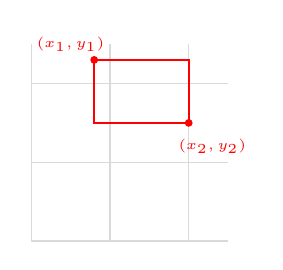
\begin{tikzpicture}[scale=1.0]
						\draw[gray!30] (0,0) grid (2.5,2.5);
						\draw[thick, red] (0.8,1.5) rectangle (2,2.3);
						\node[red, font=\tiny] at (0.5, 2.5) {$(x_1,y_1)$};
						\node[red, font=\tiny] at (2.3, 1.2) {$(x_2,y_2)$};
						\node[fill=red, circle, inner sep=1pt] at (0.8,2.3) {};
						\node[fill=red, circle, inner sep=1pt] at (2,1.5) {};
					\end{tikzpicture}
				\end{center}
			\end{block}
		\end{column}

		\begin{column}{0.5\textwidth}
			\begin{block}{Centro $(c_x, c_y, w, h)$}
				\small
				Centro, ancho y alto.
				\begin{center}
					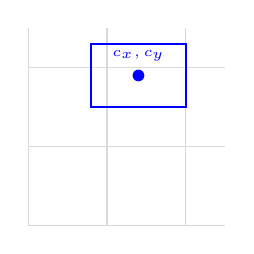
\begin{tikzpicture}[scale=1.0]
						\draw[gray!30] (0,0) grid (2.5,2.5);
						\draw[thick, blue] (0.8,1.5) rectangle (2,2.3);
						\node[fill=blue, circle, inner sep=1.5pt] at (1.4,1.9) {};
						\node[blue, font=\tiny] at (1.4, 2.15) {$c_x, c_y$};
					\end{tikzpicture}
				\end{center}
			\end{block}
		\end{column}
	\end{columns}

\end{frame}

\begin{frame}[shrink]{Conversi\'on entre Representaciones}

	Las dos representaciones son equivalentes.

	\vspace{0.4cm}

	{\small
	\begin{align*}
		c_x &= \frac{x_1 + x_2}{2}, \quad c_y = \frac{y_1 + y_2}{2}, \quad w = x_2 - x_1, \quad h = y_2 - y_1 \\[0.3cm]
		x_1 &= c_x - \frac{w}{2}, \quad y_1 = c_y - \frac{h}{2}, \quad x_2 = c_x + \frac{w}{2}, \quad y_2 = c_y + \frac{h}{2}
	\end{align*}
	}

	\vspace{0.3cm}

	\begin{block}{Almacenamiento}
		Los bounding boxes se representan como tensores de forma $(n, 4)$, donde $n$ es el n\'umero de cajas.
	\end{block}

\end{frame}

\section{Evaluaci\'on}

\begin{frame}{Intersecci\'on sobre Uni\'on (IoU)}

	La m\'etrica \textbf{IoU} cuantifica qu\'e tan bien coinciden las predicciones con la verdad.

	\vspace{0.3cm}

	\[
	\text{IoU} = \frac{\text{Intersecci\'on}}{\text{Uni\'on}}
	\]

	\vspace{0.3cm}

	\begin{center}
		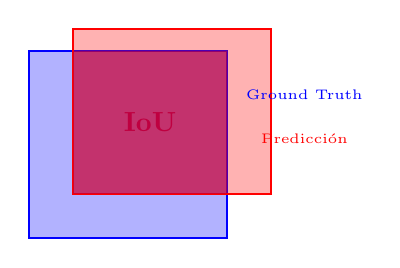
\begin{tikzpicture}[scale=1.4]
			% Ground truth (azul)
			\fill[blue, opacity=0.3] (0.5,0.5) rectangle (2.3,2.2);
			\draw[thick, blue] (0.5,0.5) rectangle (2.3,2.2);

			% Predicci\'on (rojo)
			\fill[red, opacity=0.3] (0.9,0.9) rectangle (2.7,2.4);
			\draw[thick, red] (0.9,0.9) rectangle (2.7,2.4);

			% Intersecci\'on (p\'urpura)
			\fill[purple, opacity=0.6] (0.9,0.9) rectangle (2.3,2.2);

			\node[blue, font=\tiny] at (3, 1.8) {Ground Truth};
			\node[red, font=\tiny] at (3, 1.4) {Predicci\'on};
			\node[purple, font=\tiny, font=\bfseries] at (1.6, 1.55) {IoU};
		\end{tikzpicture}
	\end{center}

	\vspace{0.2cm}

	\begin{itemize}
		\item IoU $\geq$ 0.5: Positivo verdadero (est\'andar)
		\item IoU = 1.0: Predicci\'on perfecta
	\end{itemize}

\end{frame}

\section{Paradigmas de Detecci\'on}

\begin{frame}{Tres Paradigmas de Detecci\'on}

	\begin{columns}[T]
		\begin{column}{0.33\textwidth}
			\begin{block}{Basados en Regiones}
				\small
				\begin{itemize}
					\item Proponen regiones candidatas.
					\item Clasifican y refinan.
					\item Ejemplo: Faster R-CNN
					\item Lentos pero precisos.
				\end{itemize}
			\end{block}
		\end{column}

		\begin{column}{0.33\textwidth}
			\begin{block}{Una Etapa}
				\small
				\begin{itemize}
					\item Predicci\'on directa.
					\item Ejemplo: YOLO, SSD
					\item R\'apidos pero menos precisos.
					\item Tiempo real.
				\end{itemize}
			\end{block}
		\end{column}

		\begin{column}{0.33\textwidth}
			\begin{block}{Transformers}
				\small
				\begin{itemize}
					\item Contexto global.
					\item Ejemplo: DETR
					\item Rendimiento equilibrado.
					\item Arquitectura limpia.
				\end{itemize}
			\end{block}
		\end{column}
	\end{columns}

\end{frame}

\begin{frame}{R-CNN: Inception de la Detecci\'on Profunda}

	\textbf{R-CNN} (Girshick et al., 2014) fue el primer m\'etodo exitoso con redes profundas.

	\vspace{0.3cm}

	\begin{block}{Pipeline de 4 Pasos}
		\begin{enumerate}
			\item \textbf{Propostas:} Generar \~{}2000 regiones candidatas (b\'usqueda selectiva).
			\item \textbf{CNN:} Extraer caracter\'isticas de cada regi\'on con AlexNet.
			\item \textbf{Clasificaci\'on:} Clasificar con SVM.
			\item \textbf{Regresi\'on:} Ajustar coordenadas del bounding box.
		\end{enumerate}
	\end{block}

	\vspace{0.3cm}

	\begin{alertblock}{Limitaci\'on}
		Muy lento: \~{}50 segundos por imagen (necesita 2000 pasadas).
	\end{alertblock}

\end{frame}

\begin{frame}{Arquitectura R-CNN: AlexNet de 8 Capas}
 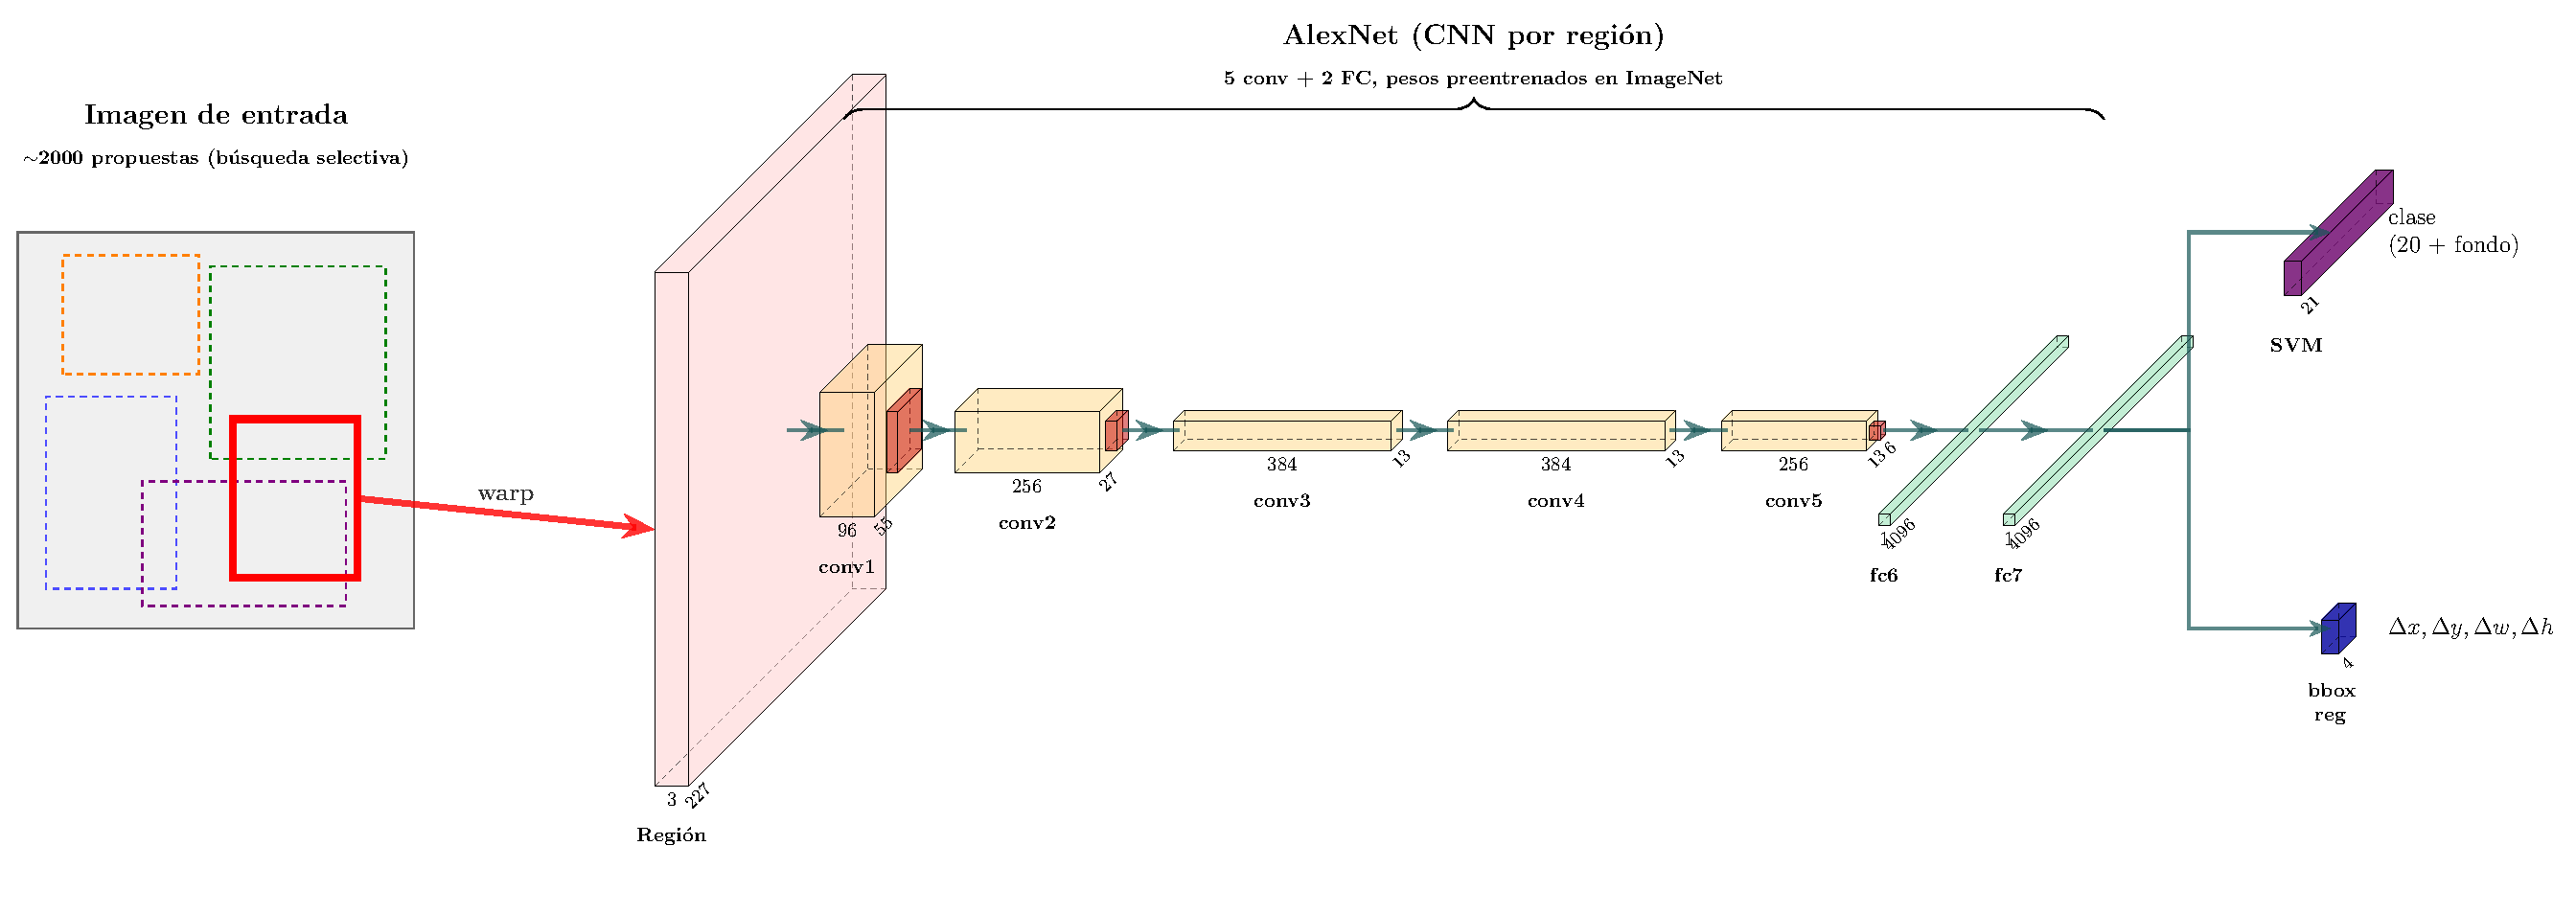
\includegraphics[width=\textwidth]{figures/alexnet_rcnn}

\end{frame}

\begin{frame}[shrink]{Arquitectura R-CNN: AlexNet de 8 Capas}

	\textbf{R-CNN utiliza AlexNet} como red convolucional base.

	\vspace{0.2cm}

	\begin{columns}[T]
		\begin{column}{0.5\textwidth}
			\begin{block}{Backbone CNN}
				\small
				\begin{itemize}
					\item \textbf{AlexNet}: 8 capas (5 conv + 3 FC)
					\item \textbf{Conv layers 1-5:}
					\begin{itemize}
						\item L1: 96 filtros, 11×11, stride 4, padding 0
						\item L2: 256 filtros, 5×5, stride 1, padding 2
						\item L3-5: 384/384/256, 3×3, stride 1, padding 1
					\end{itemize}
					\item Max pooling: 3×3, stride 2
					\item Entrada: 227×227 RGB
					\item Salida: 6×6×256 (despu\'es \'ultimas conv)
				\end{itemize}
			\end{block}
		\end{column}

		\begin{column}{0.5\textwidth}
			\begin{block}{Head (Clasificaci\'on + Regresi\'on)}
				\small
				\begin{itemize}
					\item \textbf{FC6-FC8:} 3 capas densas
					\begin{itemize}
						\item FC6: 4096 unidades
						\item FC7: 4096 unidades
						\item FC8: 21 unidades (20 clases + background)
					\end{itemize}
					\item ReLU activaci\'on entre capas
					\item Dropout: 0.5
					\item \textbf{Regresi\'on:} 4 salidas ($\Delta x, \Delta y, \Delta w, \Delta h$)
				\end{itemize}
			\end{block}
		\end{column}
	\end{columns}

\end{frame}

\begin{frame}[shrink]{Fast R-CNN: Arquitectura con RoI Pooling}

	Las mejoras posteriores aceleraron dr\'asticamente el m\'etodo original.

	\vspace{0.2cm}

	\begin{block}{Backbone: ResNet-50 o ResNet-101}
		\small
		\begin{itemize}
			\item \textbf{ResNet-50:} 50 capas en 4 bloques residuales
			\begin{itemize}
				\item Conv1: 7×7, stride 2, padding 3 (input 224×224)
				\item Residual blocks: layer1-4 con stride 2 entre bloques
				\item Bottleneck bloques: 1×1→3×3→1×1 convolutions
				\item Output stride 32 (H/W ÷ 32)
			\end{itemize}
		\end{itemize}
	\end{block}

	\vspace{0.2cm}

	\begin{columns}[T]
		\begin{column}{0.5\textwidth}
			\begin{block}{RoI Pooling}
				\small
				\begin{itemize}
					\item Aplica max pooling a cada regi\'on.
					\item Input: Feature map + coordenadas de RoI
					\item Output: 7×7×512 (uniforme)
					\item Conexiones posteriores al head
				\end{itemize}
			\end{block}
		\end{column}

		\begin{column}{0.5\textwidth}
			\begin{block}{Head Dense}
				\small
				\begin{itemize}
					\item FC6: 4096 unidades, ReLU
					\item FC7: 4096 unidades, ReLU
					\item FC8-cls: \#clases salidas
					\item FC8-reg: 4 salidas ($\Delta x, \Delta y, \Delta w, \Delta h$)
					\item Dropout: 0.5
				\end{itemize}
			\end{block}
		\end{column}
	\end{columns}

\end{frame}

\begin{frame}[shrink]{Faster R-CNN: Region Proposal Network}

	\textbf{Faster R-CNN} a\~nade RPN para propostas autom\'aticas.

	\vspace{0.2cm}

	\begin{block}{Backbone: ResNet-50/101 (igual que Fast R-CNN)}
		Entrada: imagen 1000×1000, Output: feature map H/32 × W/32
	\end{block}

	\vspace{0.2cm}

	\begin{columns}[T]
		\begin{column}{0.5\textwidth}
			\begin{block}{Region Proposal Network}
				\small
				\begin{itemize}
					\item \textbf{3×3 conv:} 512 filtros, stride 1, padding 1
					\item \textbf{Rama cls:} 1×1 conv, 2 outputs (object/background)
					\item \textbf{Rama reg:} 1×1 conv, 4 outputs ($\Delta x, \Delta y, \Delta w, \Delta h$)
					\item \textbf{Anchors:} 9 anchors por píxel (3 escalas × 3 ratios)
					\item NMS: Umbral IoU 0.7
				\end{itemize}
			\end{block}
		\end{column}

		\begin{column}{0.5\textwidth}
			\begin{block}{Head Detection}
				\small
				\begin{itemize}
					\item RoI Align (mejora de RoI Pooling)
					\item Output: 7×7×512
					\item FC6-FC7: 1024 unidades cada una
					\item FC-cls: \#clases salidas
					\item FC-reg: 4 $\times$ \#clases salidas
					\item P\'erdida multi-tarea: Lcls + $\lambda$Lreg
				\end{itemize}
			\end{block}
		\end{column}
	\end{columns}

\end{frame}

\begin{frame}{Faster R-CNN: Arquitectura Completa}
 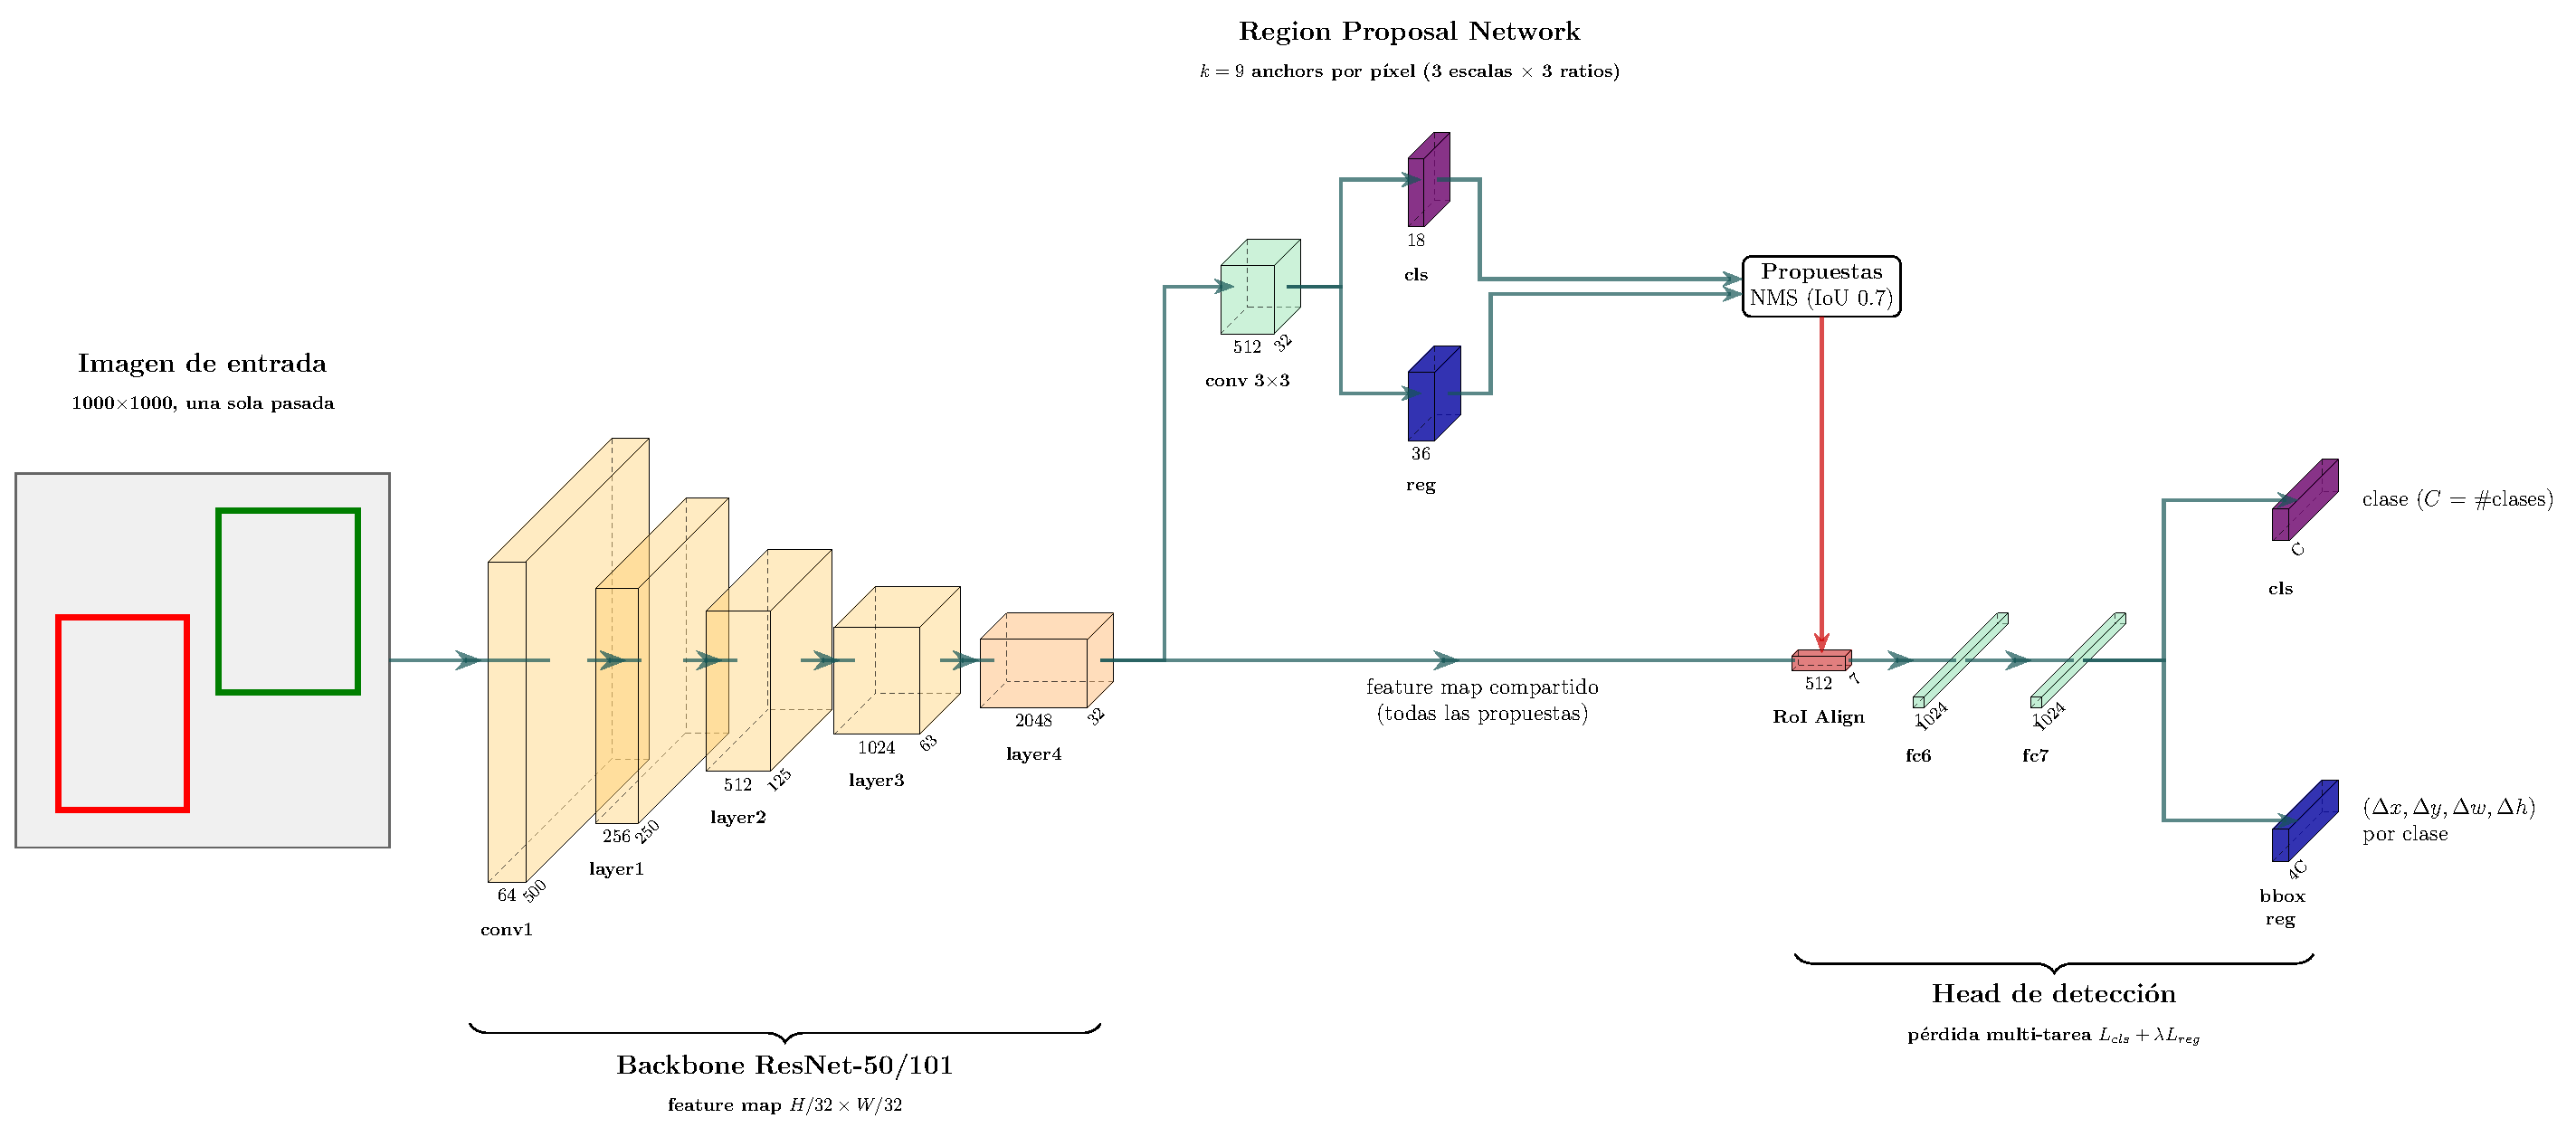
\includegraphics[width=\textwidth]{figures/faster_rcnn}
\end{frame}

\begin{frame}{YOLO: You Only Look Once}

	\textbf{YOLO} (Redmon et al., 2016) cambio el paradigma: \textbf{una sola pasada}.

	\vspace{0.3cm}

	\begin{block}{Idea: Regresi\'on Directa}
		Divide la imagen en cuadr\'icula $S \times S$ y predice:
		\begin{itemize}
			\item Confianza de objeto en cada celda.
			\item Clase del objeto.
			\item Desplazamiento del bounding box.
		\end{itemize}
	\end{block}

	\vspace{0.3cm}

	\begin{center}
		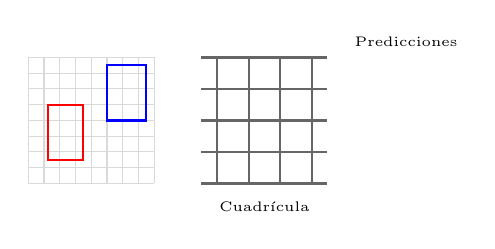
\begin{tikzpicture}[scale=1.0]
			% Imagen
			\draw[step=0.2cm, gray!30] (0,0) grid (1.6,1.6);
			\draw[thick, red] (0.25,0.3) rectangle (0.7,1);
			\draw[thick, blue] (1,0.8) rectangle (1.5,1.5);

			% Cuadr\'icula
			\draw[step=0.4cm, black!60, thick] (2.2,0) grid (3.8,1.6);
			\node[font=\tiny] at (3, -0.3) {Cuadr\'icula};

			% Predicciones
			\node[font=\tiny] at (4.8, 1.8) {Predicciones};
		\end{tikzpicture}
	\end{center}

	\begin{itemize}
		\item Ventaja: 45 FPS (tiempo real)
		\item Desventaja: Menos preciso en objetos peque\~nos
	\end{itemize}

\end{frame}

\begin{frame}[shrink]{YOLOv1: Arquitectura Completa de 24 Capas}

	\textbf{YOLOv1} utiliza una red simple pero efectiva de 24 capas convolucionales.

	\vspace{0.2cm}

	\begin{block}{Backbone Convolucional}
		\small
		\begin{itemize}
			\item \textbf{7 conv layers}: 64-128-256-512 filtros
			\begin{itemize}
				\item Conv1: 7×7, stride 2, padding 3 (input 448×448)
				\item Conv2: 3×3, stride 2, padding 1
				\item Intercaladas con max pooling 2×2, stride 2
			\end{itemize}
			\item Output: 7×7×512 (grid S=7)
			\item Activaci\'on: ReLU (excepto \'ultima capa sigmoid)
		\end{itemize}
	\end{block}

	\vspace{0.2cm}

	\begin{block}{Head Dense (Predicciones)}
		\small
		\begin{itemize}
			\item FC1: 4096 unidades, ReLU
			\item FC2: 7×7×30 = 1470 unidades
			\begin{itemize}
				\item 7×7 celdas
				\item 2 bounding boxes por celda (4 + 1 confianza = 5)
				\item 20 clases probabilidades
				\item Total: 7×7×(2×5 + 20) = 7×7×30
			\end{itemize}
		\end{itemize}
	\end{block}

\end{frame}

\begin{frame}[shrink]{YOLOv5: Arquitectura Moderna con CSPDarknet}

	\textbf{YOLOv5} introduce mejoras arquitecturales y de entrenamiento significativas.

	\vspace{0.2cm}

	\begin{columns}[T]
		\begin{column}{0.5\textwidth}
			\begin{block}{Backbone: CSPDarknet}
				\small
				\begin{itemize}
					\item \textbf{CSP:} Cross Stage Partial
					\item 5 bloques CSP con estructura residual
					\item Stride 2 entre bloques
					\item Output 3 feature maps:
					\begin{itemize}
						\item P3: H/8 × W/8 (pequeños)
						\item P4: H/16 × W/16 (medianos)
						\item P5: H/32 × W/32 (grandes)
					\end{itemize}
					\item Activaci\'on: SiLU (Swish)
				\end{itemize}
			\end{block}
		\end{column}

		\begin{column}{0.5\textwidth}
			\begin{block}{Neck: FPN}
				\small
				\begin{itemize}
					\item \textbf{Feature Pyramid Network}
					\item Conexiones up-sampling + down-sampling
					\item Fusi\'on multi-escala de caracter\'isticas
					\item Concatenaci\'on + 1×1 convs
				\end{itemize}
			\end{block}
		\end{column}
	\end{columns}

	\vspace{0.2cm}

	\begin{block}{Head: Predicciones Multi-Escala}
		\small
		3 cabezas de detecci\'on (una por escala): Conv 1×1 por escala, output (x,y,w,h,conf,cls1,...,cls80)
	\end{block}

\end{frame}

\begin{frame}{Yolov5: Arquitectura Completa}
 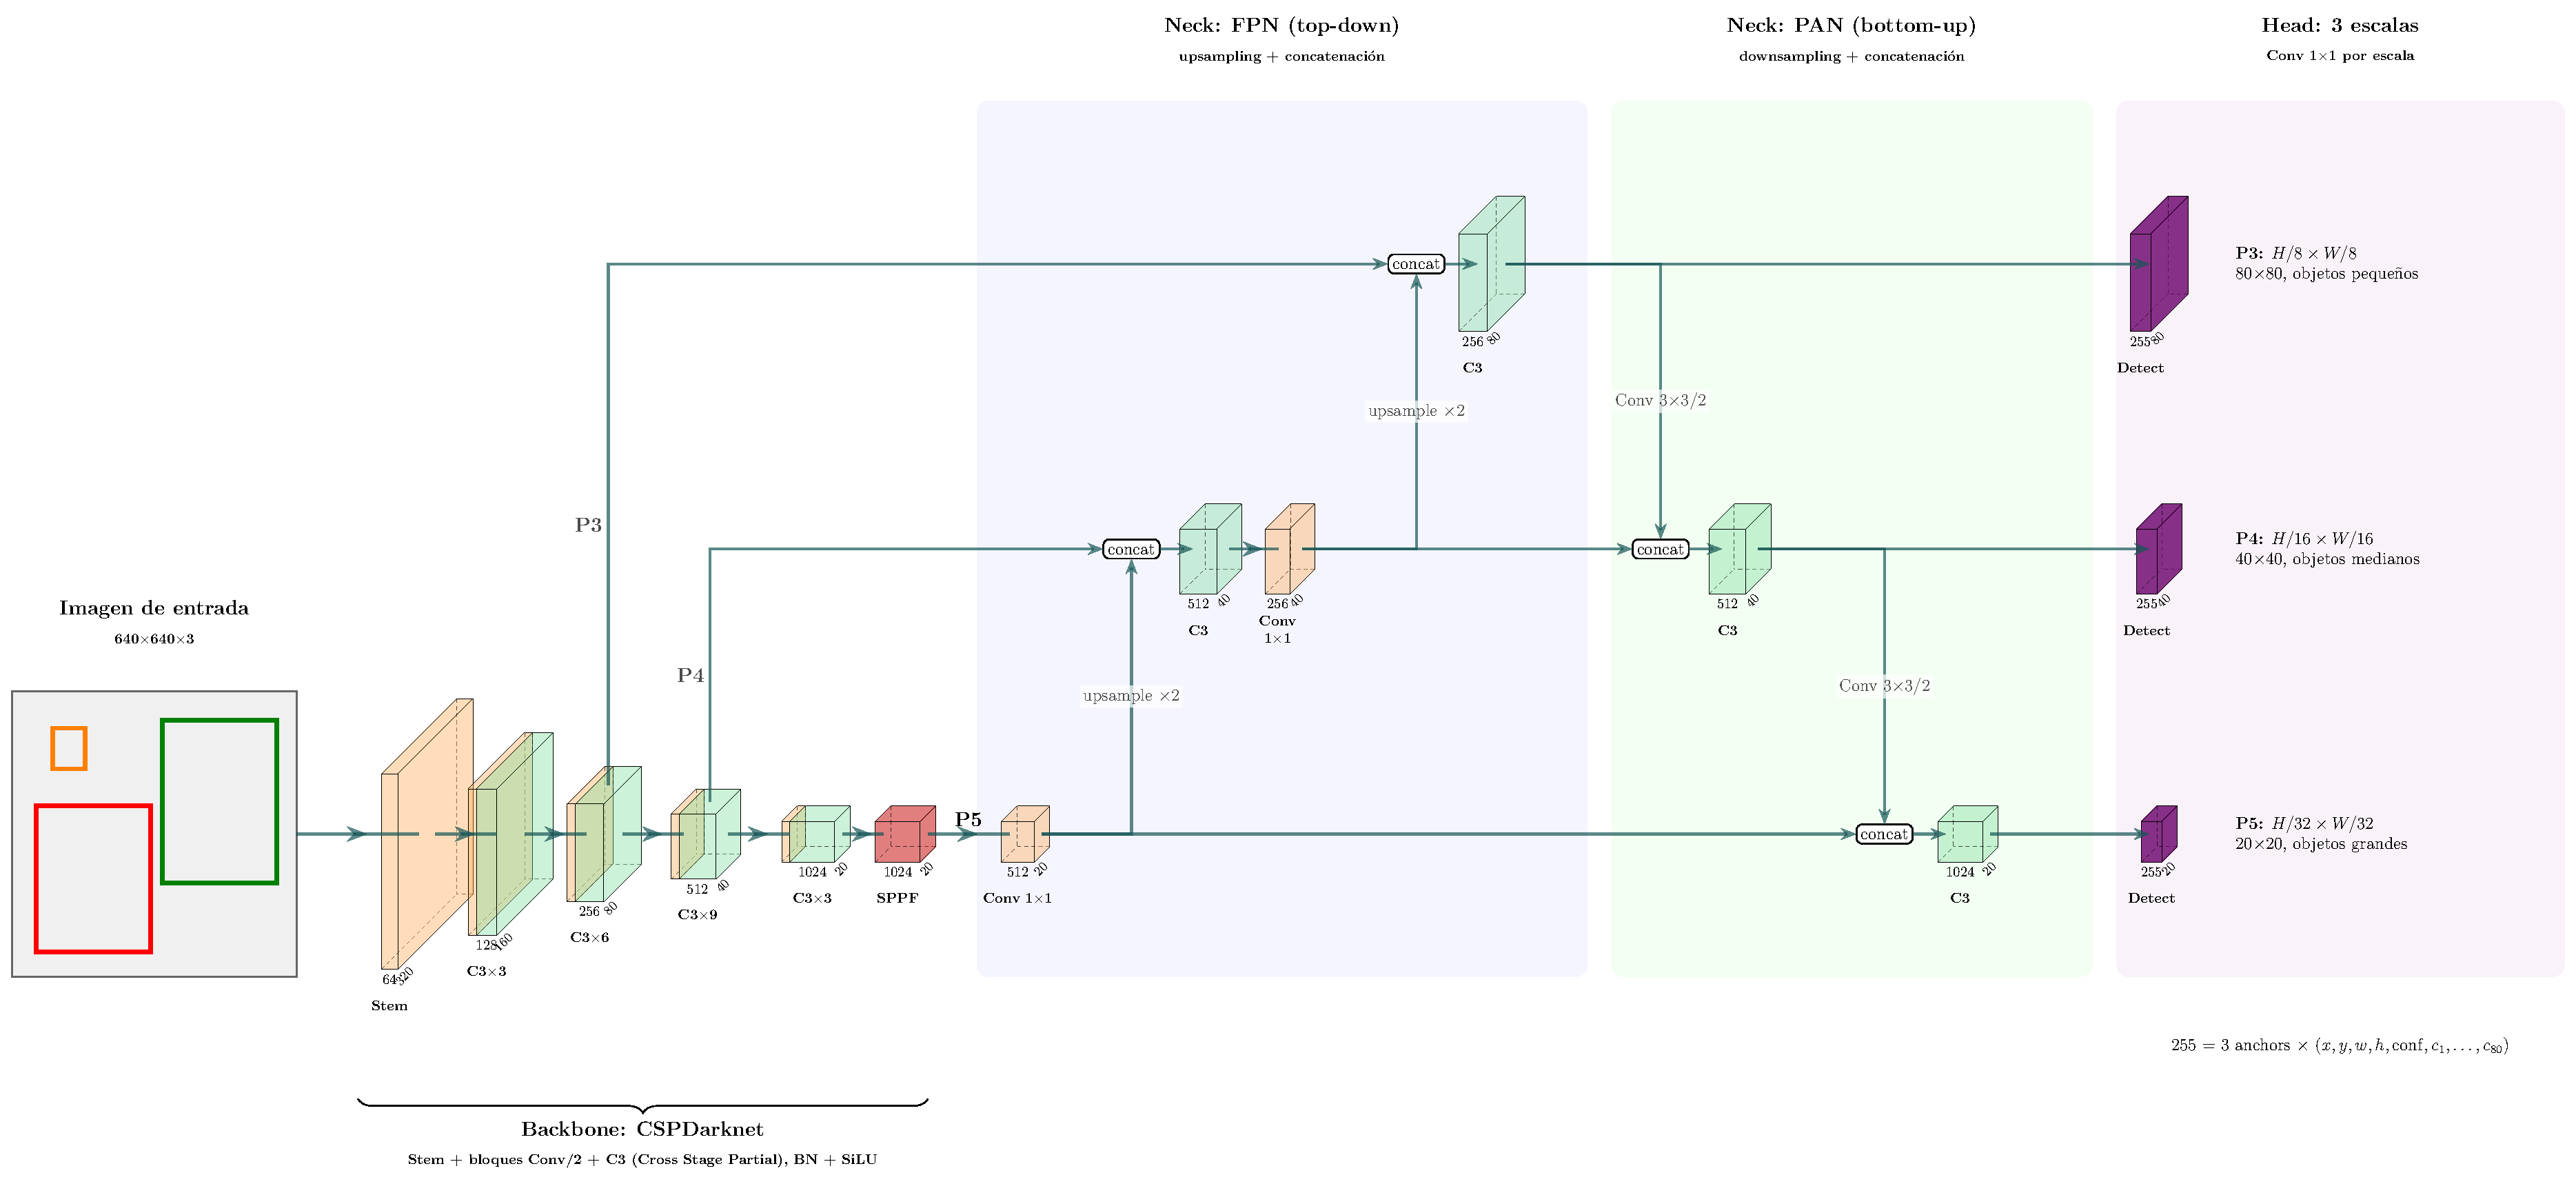
\includegraphics[width=\textwidth]{figures/yolov5}
\end{frame}

\begin{frame}[shrink]{SSD300: Arquitectura Multi-Escala con VGG-16}

	\textbf{SSD300} usa VGG-16 truncado como backbone base.

	\vspace{0.15cm}

	\begin{columns}[T]
		\begin{column}{0.5\textwidth}
			\begin{block}{Backbone: VGG-16 Truncado}
				\small
				\begin{itemize}
					\item VGG-16: 16 capas conv
					\item Primeras 13 conv layers
					\begin{itemize}
						\item Bloques de 2-3 convs 3×3
						\item Stride 1, max pool stride 2
						\item Canales: 64-128-256-512
					\end{itemize}
					\item \textbf{Remover:} \'Ultimas FC layers
					\item Input: 300×300 RGB
					\item Output: 38×38×512
				\end{itemize}
			\end{block}
		\end{column}

		\begin{column}{0.5\textwidth}
			\begin{block}{Capas Adicion. Multi-Escala}
				\small
				\begin{itemize}
					\item Conv 1×1: 1024 filtros
					\item Conv 1×1: 1024 filtros
					\item Series de conv 3×3 stride 2
					\begin{itemize}
						\item Stride 2: 512
						\item Stride 2: 256
						\item Stride 2: 256
						\item Stride 2: 256
					\end{itemize}
					\item Feature maps:
					\begin{itemize}
						\item 38×38 (VGG)
						\item 19×19, 10×10, 5×5, 3×3, 1×1
					\end{itemize}
				\end{itemize}
			\end{block}
		\end{column}
	\end{columns}

\end{frame}

\begin{frame}[shrink]{SSD: Heads de Detecci\'on Multi-Escala}

	Para cada feature map, se aplican convoluciones 3×3 peque\~nas.

	\vspace{0.15cm}

	\begin{block}{Predicci\'on por Escala}
		\small
		Para cada feature map de tamaño $m \times m$:
		\begin{itemize}
			\item \textbf{Conv 3×3:} Aplicada a cada posici\'on spatial
			\item Para cada anchor: predice $(x, y, w, h, c_0, ..., c_{19})$
			\item M\'ultiples anchors por posici\'on (4-6 formas y escalas)
			\item Salida: $m \times m \times (\text{\#anchors} \times (4 + \text{\#clases}))$
		\end{itemize}
	\end{block}

	\vspace{0.15cm}

	\begin{block}{Ejemplo SSD300}
		\small
		\begin{itemize}
			\item \textbf{38×38:} 4 anchors $\to$ 38×38×96 (4 coords + 20 clases) × 4
			\item \textbf{19×19:} 6 anchors $\to$ 19×19×144
			\item \textbf{10×10:} 6 anchors $\to$ 10×10×144
			\item \textbf{5×5:} 6 anchors $\to$ 5×5×144
			\item \textbf{3×3:} 4 anchors $\to$ 3×3×96
			\item \textbf{1×1:} 4 anchors $\to$ 1×1×96
			\item \textbf{Total:} \~{}8732 predicciones de bounding box
		\end{itemize}
	\end{block}

\end{frame}

\begin{frame}{SSD300: Arquitectura Completa}
 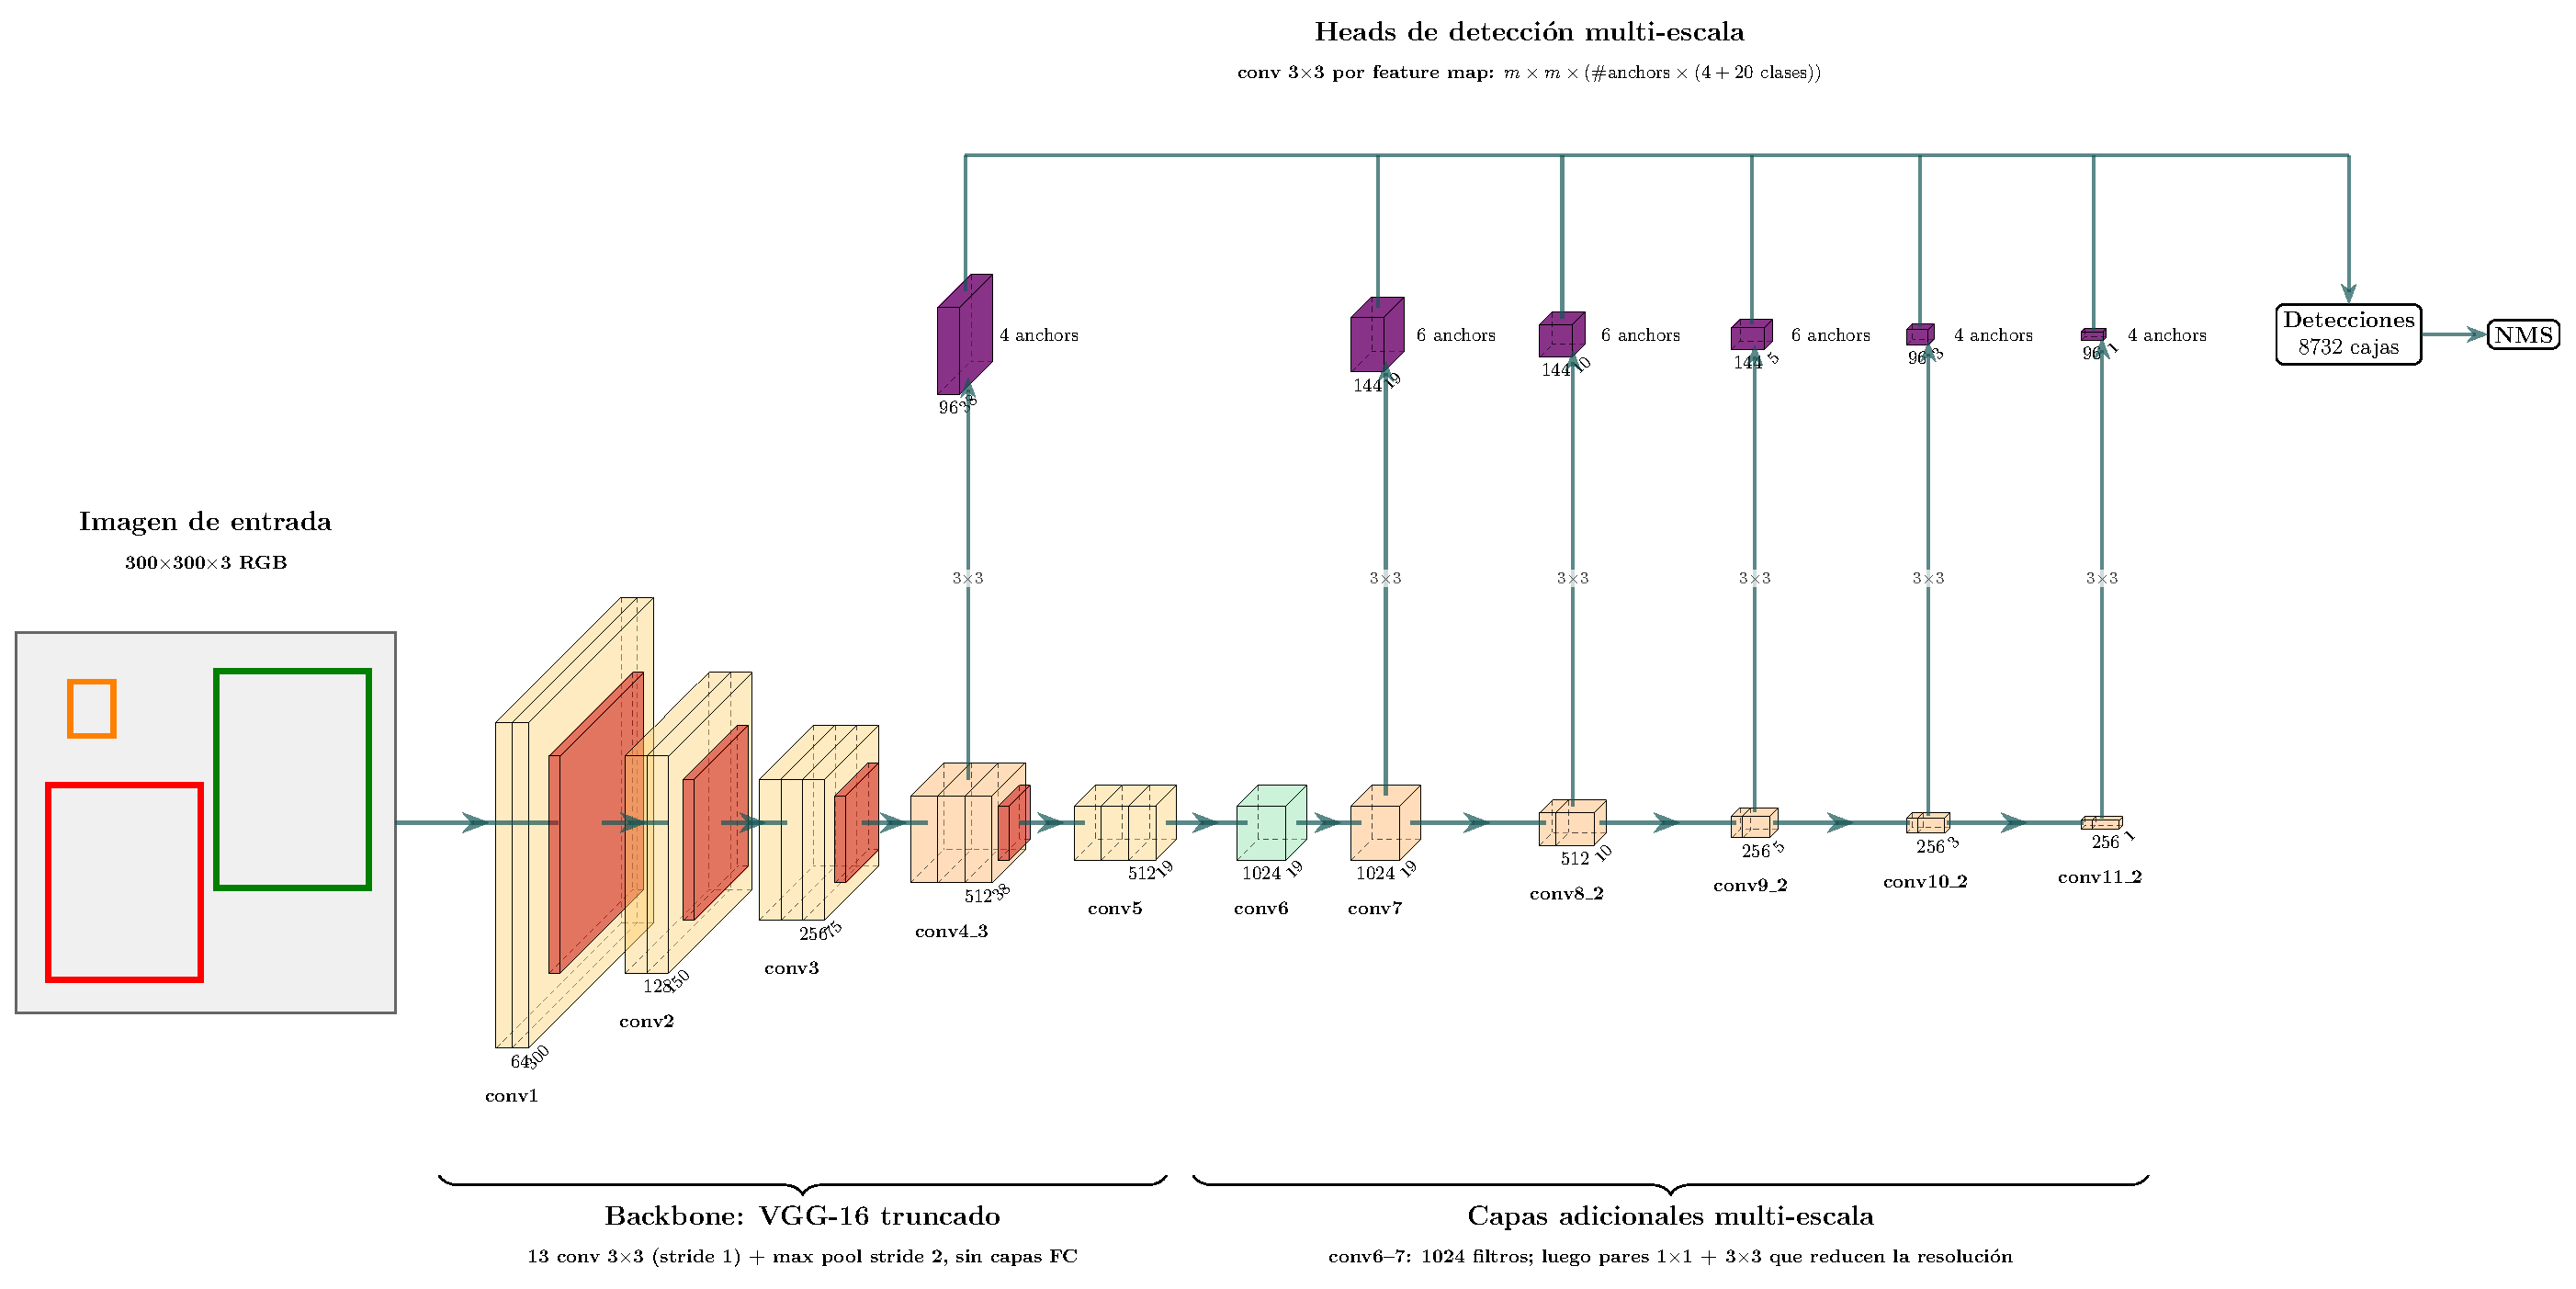
\includegraphics[width=\textwidth]{figures/ssd300}
\end{frame}

\section{Arquitecturas Modernas}

\begin{frame}{DETR: Detection Transformer - Cambio de Paradigma}

	\textbf{DETR} (Carion et al., 2020) reformula detecci\'on como \textbf{predicci\'on directa de conjuntos}.

	\vspace{0.3cm}

	\begin{block}{Cambio de Paradigma}
		\begin{itemize}
			\item \textbf{Enfoque tradicional:} Genera propostas de regiones, filtra, refina (multi-etapa).
			\item \textbf{DETR:} Predice directamente un conjunto fijo de detecciones en paralelo.
			\item Trata detecci\'on como un problema de asignaci\'on de conjuntos.
			\item Elimina componentes manuales como NMS, anchor boxes.
		\end{itemize}
	\end{block}

	\vspace{0.3cm}

	\begin{block}{Arquitectura}
		\begin{itemize}
			\item \textbf{Encoder CNN:} Extrae caracter\'isticas espaciales.
			\item \textbf{Transformer:} Captura relaciones globales.
			\item \textbf{Decoder:} Predice clase y bbox para N objetos.
		\end{itemize}
	\end{block}

\end{frame}

\begin{frame}[shrink]{Predicci\'on Basada en Conjuntos}

	DETR predice un conjunto de N detecciones (donde N >> n\'umero real de objetos).

	\vspace{0.3cm}

	\begin{block}{Formulaci\'on del Problema}
		\begin{itemize}
			\item Predice: $\hat{\mathcal{Y}} = \{(\hat{c}_i, \hat{b}_i)\}_{i=1}^{N}$ donde $\hat{c}_i$ es clase y $\hat{b}_i$ es bounding box.
			\item $N$ es fijo (ej. N=100) >> n\'umero real de objetos.
			\item Muchas predicciones ser\'an clase ``vac\'io'' (no-object).
			\item No hay orden: dos permutaciones del conjunto tienen el mismo significado.
		\end{itemize}
	\end{block}

	\vspace{0.3cm}

	\begin{alertblock}{Ventaja Clave}
		Al ser un conjunto, el orden no importa. Esto permite decodificaci\'on \textbf{paralela} en lugar de secuencial.
	\end{alertblock}

\end{frame}

\begin{frame}[shrink]{Emparejamiento Bip\'artito y el Algoritmo H\'ungaro}

	El desaf\'io: asignar predicciones a objetos verdaderos de forma \'optima.

	\vspace{0.3cm}

	\begin{block}{Problema de Asignaci\'on}
		\begin{itemize}
			\item Tenemos N predicciones y (t\'ipicamente) mucho menos objetos verdaderos.
			\item Necesitamos encontrar permutaci\'on \'optima $\sigma \in \mathcal{S}_N$.
			\item Objetivo: minimizar costo de emparejamiento total.
		\end{itemize}
	\end{block}

	\vspace{0.2cm}

	{\small
	\[
	\hat{\sigma} = \arg\min_{\sigma} \sum_{i=1}^{N} \mathcal{L}_{\text{match}}(y_i, \hat{y}_{\sigma(i)})
	\]
	}

	\begin{block}{Soluci\'on: Algoritmo H\'ungaro}
		\begin{itemize}
			\item Resuelve el problema de asignaci\'on \'optima en tiempo polinomial.
			\item Cada predicci\'on se empareja con un objeto verdadero (o vac\'io).
			\item Evita duplicados: una predicci\'on = un objeto o vac\'io.
			\item Eficiencia: $O(n^3)$ es manejable para N=100.
		\end{itemize}
	\end{block}

\end{frame}

\begin{frame}[shrink]{Costo de Emparejamiento: Combinaci\'on de Clase y Localizaci\'on}

	El costo de emparejamiento combina informaci\'on de clasificaci\'on y bbox.

	\vspace{0.2cm}

	{\small
	\[
	\mathcal{L}_{\text{match}}(y_i, \hat{y}_{\sigma(i)}) = -\mathbb{1}_{c_i \neq \emptyset} \hat{p}_{\sigma(i)}(c_i) + \mathbb{1}_{c_i \neq \emptyset} \mathcal{L}_{\text{box}}(b_i, \hat{b}_{\sigma(i)})
	\]
	}

	\vspace{0.2cm}

	\begin{block}{Componentes}
		\begin{itemize}
			\item \textbf{T\'ermino de clasificaci\'on:} $-\hat{p}_{\sigma(i)}(c_i)$ = probabilidad negativa de clase correcta.
			\item \textbf{T\'ermino de caja:} Solo se aplica si $c_i \neq \emptyset$ (hay un objeto real).
			\item Los indicadores $\mathbb{1}_{c_i \neq \emptyset}$ aseguran que no se penaliza perder ``no-objetos''.
		\end{itemize}
	\end{block}

	\vspace{0.2cm}

	\begin{alertblock}{Caracter\'istica Clave}
		Diferente a m\'etodos tradicionales: no usa NMS post-procesamiento, sino matching \'optimo durante entrenamiento.
	\end{alertblock}

\end{frame}

\begin{frame}[shrink]{P\'erdida H\'ungara: Entrenamiento del Modelo}

	Despu\'es del emparejamiento \'optimo, se calcula la p\'erdida total para backpropagation.

	\vspace{0.2cm}

	{\small
	\[
	\mathcal{L}_{\text{Hungarian}} = \sum_{i=1}^{N} \left[-\log \hat{p}_{\hat{\sigma}(i)}(c_i) + \mathbb{1}_{c_i \neq \emptyset} \mathcal{L}_{\text{box}}(b_i, \hat{b}_{\hat{\sigma}(i)})\right]
	\]
	}

	\vspace{0.2cm}

	\begin{block}{Componentes}
		\begin{itemize}
			\item \textbf{P\'erdida de clasificaci\'on:} Entrop\'ia cruzada en probabilidades de clase predichas.
			\item \textbf{P\'erdida de bbox:} Solo se aplica a objetos reales (no a predicciones vac\'ias).
			\item \textbf{Ponderaci\'on:} Se reduce el peso de ``no-objeto'' por factor $\lambda = 10$ para evitar dominancia (99\% de predicciones ser\'an vac\'ias).
		\end{itemize}
	\end{block}

	\vspace{0.2cm}

	\begin{alertblock}{Manejo del Desbalance de Clases}
		La mayor\'ia de predicciones son vac\'ias, por eso se pondera: $\mathcal{L}_{\emptyset} = 0.1 \times \mathcal{L}_{\text{matched}}$.
	\end{alertblock}

\end{frame}

\begin{frame}[shrink]{P\'erdida de Caja: Combinaci\'on de GIoU y L1}

	Para localizaci\'on de bounding boxes, se combina dos p\'erdidas complementarias.

	\vspace{0.2cm}

	{\small
	\[
	\mathcal{L}_{\text{box}} = \lambda_{\text{iou}} \mathcal{L}_{\text{GIoU}} + \lambda_{L1} \left\| b_i - \hat{b}_{\hat{\sigma}(i)} \right\|_1
	\]
	}

	\vspace{0.2cm}

	\begin{columns}[T]
		\begin{column}{0.5\textwidth}
			\begin{block}{P\'erdida GIoU}
				\small
				\begin{itemize}
					\item \textit{Generalized IoU}: resuelve problema de IoU cuando boxes no se superponen.
					\item \textbf{Escala invariante}: penalizaci\'on homog\'enea para cajas grandes y peque\~nas.
					\item Rango: $[-1, 1]$ ($-1$ = cajas opuestas, $1$ = perfectas).
				\end{itemize}
			\end{block}
		\end{column}

		\begin{column}{0.5\textwidth}
			\begin{block}{P\'erdida L1}
				\small
				\begin{itemize}
					\item Captura precisi\'on en coordenadas (pixeles).
					\item \textbf{Sensible a escala}: mejor para ajustes finos.
					\item Complementa GIoU: GIoU para forma, L1 para precisi\'on.
				\end{itemize}
			\end{block}
		\end{column}
	\end{columns}

	\vspace{0.2cm}

	\begin{block}{Ponderaci\'on}
		T\'ipicamente: $\lambda_{\text{iou}} = 2$, $\lambda_{L1} = 5$ para balancear contribuciones.
	\end{block}

\end{frame}

\begin{frame}[shrink]{DETR: Arquitectura Completa}

	\textbf{DETR} combina backbone CNN con transformers para predicci\'on de conjuntos.

	\vspace{0.15cm}

	\begin{columns}[T]
		\begin{column}{0.33\textwidth}
			\begin{block}{Backbone CNN}
				\small
				\begin{itemize}
					\item ResNet-50 o ResNet-101
					\item 50/101 capas conv
					\item Stride 32
					\item Input: 800×1066 ($\sim$3 MP)
					\item Output: 25×34×2048 features
				\end{itemize}
			\end{block}
		\end{column}

		\begin{column}{0.33\textwidth}
			\begin{block}{Encoder Transformer}
				\small
				\begin{itemize}
					\item 6 capas de transformer
					\item Multi-head attention: 8 heads
					\item Hidden: 256 dims
					\item FFN: 2048 dims
					\item Positional encoding: sinusoidal
					\item Dropout: 0.1
				\end{itemize}
			\end{block}
		\end{column}

		\begin{column}{0.33\textwidth}
			\begin{block}{Decoder Transformer}
				\small
				\begin{itemize}
					\item 6 capas de transformer
					\item Multi-head attention: 8 heads
					\item Hidden: 256 dims
					\item FFN: 2048 dims
					\item \textit{Learned queries}: N=100
					\item Self-attention + cross-attention
				\end{itemize}
			\end{block}
		\end{column}
	\end{columns}

\end{frame}

\begin{frame}[shrink]{DETR: Heads de Clasificaci\'on y Regresi\'on}

	Despu\'es del decoder, heads espec\'ificos predicen clases y bboxes.

	\vspace{0.15cm}

	\begin{columns}[T]
		\begin{column}{0.5\textwidth}
			\begin{block}{Head de Clasificaci\'on}
				\small
				\begin{itemize}
					\item Input: Decoder output, 256D por query
					\item 3 FC layers:
					\begin{itemize}
						\item FC1: 256D
						\item FC2: 256D
						\item FC3: (num\_classes + 1)D
					\end{itemize}
					\item +1 para clase ``sin objeto''
					\item Softmax: probabilidades
					\item Comparte pesos entre queries
				\end{itemize}
			\end{block}
		\end{column}

		\begin{column}{0.5\textwidth}
			\begin{block}{Head de Regresi\'on}
				\small
				\begin{itemize}
					\item Input: Decoder output, 256D
					\item 3 FC layers:
					\begin{itemize}
						\item FC1: 256D
						\item FC2: 256D
						\item FC3: 4D (x, y, w, h)
					\end{itemize}
					\item Regresi\'on directa (sin sigmoid)
					\item Pesos compartidos entre queries
					\item Normalizaci\'on: coords relativo a imagen
				\end{itemize}
			\end{block}
		\end{column}
	\end{columns}

\end{frame}

\begin{frame}{Ventajas de la Formulaci\'on de Conjuntos}

	\begin{block}{Simplicidad Conceptual}
		\begin{itemize}
			\item Un modelo unificado: no necesita componentes separados (RPN, NMS, etc.).
			\item Arquitectura extremo-a-extremo entrenable.
			\item Formulaci\'on matem\'atica clara y elegante.
		\end{itemize}
	\end{block}

	\vspace{0.3cm}

	\begin{block}{Ventajas Pr\'acticas}
		\begin{itemize}
			\item \textbf{Sin NMS:} El matching \'optimo reemplaza el post-procesamiento manual.
			\item \textbf{Decodificaci\'on paralela:} Todos los N objetos se predicen simult\'aneamente.
			\item \textbf{Menos hip\'otesis manuales:} No requiere dise\~no de anchors, ratios, escalas.
			\item \textbf{Generalizaci\'on:} F\'acilmente extensible a panop\'tica, instancia, etc.
		\end{itemize}
	\end{block}

\end{frame}

\begin{frame}{DETR: Arquitectura Completa}
 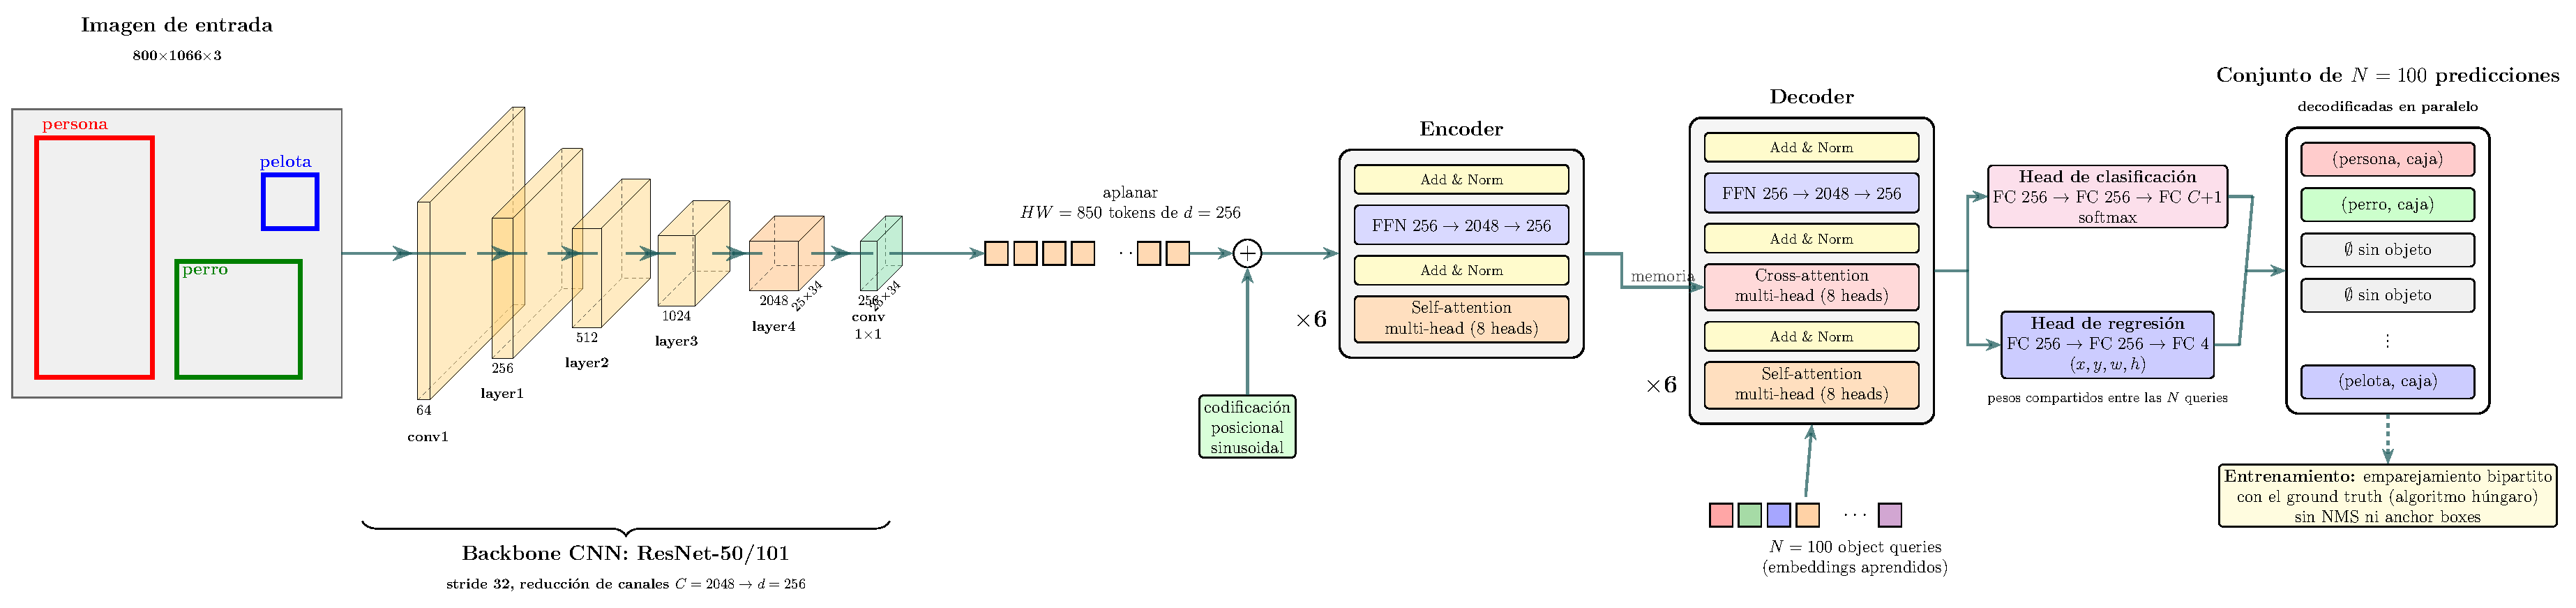
\includegraphics[width=\textwidth]{figures/detr}
\end{frame}

\begin{frame}{Evoluci\'on Reciente}

	La evoluci\'on de YOLO demuestra la importancia de la \textbf{optimizaci\'on arquitectural y de entrenamiento}.

	\vspace{0.3cm}

	\begin{block}{Mejoras en YOLOv5}
		\begin{itemize}
			\item \textbf{Backbone optimizado:} CSPDarknet con conexiones residuales mejoradas.
			\item \textbf{Feature Pyramid Network (FPN):} Extracci\'on multi-escala eficiente.
			\item \textbf{Activaciones mejoradas:} Reemplazo de ReLU con activaciones m\'as sofisticadas.
			\item \textbf{Data augmentation agresiva:} Mosaic augmentation, mixup.
			\item Logra 50.2 mAP@0.5:0.95 en COCO (competitivo con Faster R-CNN).
		\end{itemize}
	\end{block}

	\vspace{0.3cm}

	\begin{block}{Trend Actual: Eficiencia}
		\begin{itemize}
			\item M\'etodos ligeros para dispositivos m\'oviles y edge.
			\item Compresi\'on de modelos: pruning, quantizaci\'on, destilaci\'on.
			\item Trade-off precisi\'on-velocidad mejor investigado.
		\end{itemize}
	\end{block}

\end{frame}

\section{Conclusiones}

\begin{frame}{Conclusiones y Perspectivas}

	\begin{itemize}
		\item \textbf{Detecci\'on de objetos} es fundamental en visi\'on computacional y aplicaciones del mundo real.

		\vspace{0.3cm}

		\item Tres paradigmas con trade-offs claros:
		\begin{itemize}
			\item Basados en regiones $\to$ m\'axima precisi\'on.
			\item Una etapa $\to$ m\'axima velocidad.
			\item Transformers $\to$ arquitectura m\'as limpia.
		\end{itemize}

		\vspace{0.3cm}

		\item \textbf{M\'etricas:} IoU (localizaci\'on), mAP (desempe\~no), FPS (velocidad).

		\vspace{0.3cm}

		\item \textbf{Fronteras:} Fusi\'on multi-modal, detecci\'on 3D, video, objetos peque\~nos.

		\vspace{0.3cm}

		\item Elecci\'on de m\'etodo seg\'un dominio y restricciones de recursos.
	\end{itemize}

\end{frame}

\end{document}
